\chapter{Paper 1}\label{sc:p1}
\textbf{\Large Analog Modulo Integrator For Use In Open-Loop Sigma-Delta
  Modulators}\\
\indent Carsten Wulff, {\O}ystein Knauserud, Trond Ytterdal\\
\indent In proceedings of the 24th NORCHIP Conference, 2006.\\
\indent Nov. 2006 Pages 125 - 128\\
\indent Digital Object Identifier 10.1109/NORCHP.2006.329259 \\

\renewcommand\myfigname{p3fig:}
\renewcommand\myeqname{p3eq:}

\section*{Errata}
\begin{itemize}
\item Section 4.4. second paragraph, 3`rd to last line: altough $\rightarrow$ although
\end{itemize}

%------------------------------------------------------------------------
\begin{abstract}
%------------------------------------------------------------------------
%\section{Abstract}
A switched-capacitor analog modulo integrator is presented. This analog modulo
integrator makes it possible to design  
an Open-Loop Sigma-Delta Modulator (OLSDM). The theory of OLSDM and
analog modulo integration is explained and verified through simulation.


\end{abstract}
%\myfootnote{Financial support from the Norwegian Research Council through the
%project Smart Microsystems for Diagnostic Imaging in Medicine (project
%number 159559/130) and the project ASICs for Microsystems (project
%number 133952/420) is gratefully acknowledged. }
%-------------------------------------------------------
\section{Introduction}
%-------------------------------------------------------
Sigma-Delta modulators have become a natural choice for analog
to digital conversion in applications with low to medium bandwidth
and high resolution. They are used in applications from high
resolution instrumentation systems to ADSL communication systems. The purpose of the Sigma-Delta modulator is to shape the
quantization error such that the spectral density of the quantization
noise is non-uniform, the quantization error can for example be
high-pass or bandpass filtered. 

The Low-pass Conventional Sigma-Delta Modulator (LC-SDM) in its simplest form consists of an
integrator followed by a quantizer. The quantized signal is fed back
to the input through a digital-to-analog converter and subtracted from
the input. The transfer function of the modulator will be different for the
input signal and the quantization error of the quantizer. The input
signal will normally undergo an integration followed by a
differentiation and have a transfer function close to one. The quantization error will be
differentiated and thus high pass
filtered. 

Ideally this system could be implemented by an integrator
followed by a quantizer and a differentiator. However, an ideal integrator
has infinite DC gain, and with limited input swing in analog electronic
circuits, an ideal integrator is not possible to implement. This is
the reason why feedback is used, the feedback serves to
limit the signal swing. 

Another approach to \sd modulators is the Frequency
Sigma-Delta  Modulator (FSDM) \cite{hovin97}. Here 
an amplitude to frequency modulator was used instead of an integrator, similar to what was
suggested in \cite{claasen80}. It was shown in \cite{hovin97} that the 
preprocessing in FSDM is equivalent to modulo integration. 

In \cite{wisland02} they introduced the
non-feedback Sigma-Delta digital-to-analog converter. Here the
integrator was implemented as a digital modulo integrator.

This paper introduces an analog modulo integrator for use in 
OLSDM. The outline of this paper is as follows.
Section \ref{p3modolsd} explains that OLSDM are mathematically equivalent to LC-SDM.
In Section \ref{p3modint} the analog switched-capacitor modulo
integrator is presented, to our knowledge, it is the first of its
kind. System simulations in Section \ref{p3simulation} of the OLSDM 
verify the theory. 

%-------------------------------------------------------
\section{Open Loop Sigma-Delta Modulator} \label{p3modolsd}
%-------------------------------------------------------

%-------------------------------------------------------
\subsection{Proof of Equivalence }
%------------------------------------------------------- 
The equivalence of LC-SDM and OLSDM was shown in \cite{wisland02}. 
We endeavor to explain the equivalence in a more intuitive way. 

The OLSDM has been modeled as a quasi-linear system. Quasi-linear
since the modulo integration and modulo differentiation are stepwise linear.
The quantizer has been modeled as a linear addition of noise. Figure
\ref{p3fig:modolsd} shows the complete modulator. It should
be noted that this system is similar to the system presented in
Figure 1 in \cite{claasen80}, but they used a form of FM
modulation to implement the modulo integration. 

\begin{figure}[ht]
%  \begin{minipage}[b]{0.45\textwidth}
\centering 
 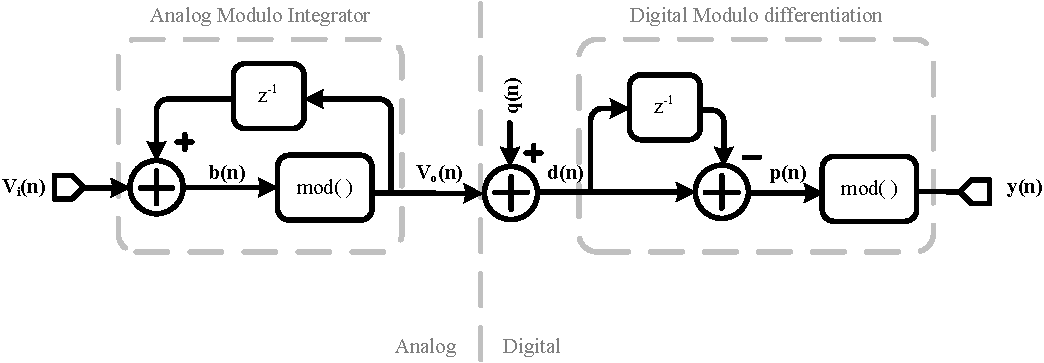
\includegraphics[width=\myfigwidth]{graphics/modolsd}
  \caption{Quasi-linear model of OLSDM}
  \label{p3fig:modolsd}
%  \end{minipage}
\end{figure}

We define the previous output from the integrator as
\eqn{
V_o(n-1) \in \langle -V_{ref}, V_{ref} \rangle
}
and the input signal as
\eqn{
\label{p3eq:rangeinput}
V_i(n) \in \langle -V_{ref}, V_{ref} \rangle
}
where $V_{ref}$ is the reference voltage.

We know that after integration, but before the modulo operation, we get
\eqn{
\label{p3eq:modintb}
b(n) = V_i(n) + V_o(n-1)
}
where $b(n)$ will be bounded by
\eqn{
b(n) \in \langle -V_{r}, V_{r} \rangle
}
where $V_r = 2V_{ref}$.
The modulo operation is used to reduce the output swing to $V_o(n) \in \langle
-V_{ref}, V_{ref} \rangle$. The modulo operation subtracts or adds
 $V_r$, depending on the value of the
summation in \req{modintb}.
The next output from the integrator can be
written as 
\begin{numcases}{V_o(n) = }
\label{p3eq:modint}
b(n) + V_r & $b(n) \in \langle -V_r, -V_{ref}]$\nonumber\\ 
b(n)  & $b(n) \in \langle -V_{ref} , V_{ref} \rangle$ \nonumber\\
b(n) - V_r & $b(n) \in [ V_{ref}, V_r \rangle$
\end{numcases}
After quantization the input to differentiation will be
\eqna{
d(n) &{}={}& V_o(n)+ q(n)\nonumber\\
d(n-1) &{}={}& V_o(n-1) + q(n-1)
}
where $q(n), q(n-1)$ are the quantization errors. 
The the output of the differentiator is
\eqn{
\label{p3eq:z(n)}
z(n) = d(n) - d(n-1)
}
If we in \req{z(n)} insert for $d(n)$, $d(n-1)$, $V_o(n)$ and set $e(n) = q(n)-q(n-1)$ the expression becomes
\begin{numcases}{z(n) = }
\label{p3eq:z2}
V_i(n) + V_r + e(n) &$V_i(n) \in \langle -V_{ref} , 0 \rangle$\nonumber\\
V_i(n) + e(n) &$V_i(n) \in \langle -V_{ref} , V_{ref} \rangle$\nonumber\\
V_i(n) - V_r + e(n) &$V_i(n) \in \langle 0 , V_{ref}  \rangle$
\end{numcases}
%The boundaries of $z(n)$, if we ignore quantization error, are given by
%\begin{numcases}{z(n) = }
%\label{p3eq:z3}
%V_i(n) + V_r  &$z(n) \in \langle V_{ref} , V_{r} \rangle$\nonumber\\
%V_i(n)  &$z(n) \in \langle -V_{ref} , V_{ref} \rangle$\nonumber\\
%V_i(n) - V_r  &$z(n) \in \langle -V_r , -V_{ref}  \rangle$
%\end{numcases}
Thus, the output of the modulator is
\begin{numcases}{y(n) = }
\label{p3eq:yn}
V_i(n) + V_r - V_r +e(n)  \nonumber\\
V_i(n) +e(n) \nonumber\\
V_i(n) -V_r +V_r + e(n) 
\end{numcases}
and for all cases in \req{yn}, $y(n) \in \langle -V_{ref} , V_{ref}
\rangle $, if we ignore the quantization error.
This gives us the well known equations
\eqn{
\frac{y(z)}{V_i(z)} = 1 \:,\:
\frac{y(z)}{q(z)} = 1- z^{-1}
}
The transfer function from the input signal to the output is one, which
is the same as for a LC-SDM (often the transfer function of a LC-SDM from input to
  output contains a time delay, $y(z)/V_i(z) = z^{-1}$ ). The quantization error is
differentiated, thus first order high pass filtered. This proof can be
extended to higher order modulators. 


%-------------------------------------------------------
%\subsection{OLSDM example }
%------------------------------------------------------- 

%An example of a conversion using the OLSDM can be seen in Figure
% \ref{p3fig:example}. Here the signals within the modulator are shown with
%their respective sample index, $n$ and $n-1$. In this example the
% quantization error is ignored for clarity, however it is shown as
%noise on the signals after quantization. The reference assigned
% an arbitrary value of $V_{ref}=3$. This value, and the other values
% in this example,  are chosen to
% correspond to the number of stacked squares in Figure \ref{p3fig:example}.  The input signal is 
%\eqn{V_i(n)  = 3 -\Delta }
%where $\Delta$ is a small value so \req{rangeinput} is satisfied. 
%After integration $b(n)$ will be given by
%\eqn{b(n) = V_i(n) + V_o(n-1) = (3 - \Delta) + 2 = 5 - \Delta}
%The output of the modulo integrator, $V_o(n)$, is
%\eqn{V_o(n) = b(n) - V_r = (5 - \Delta) -6 = -1 - \Delta}
%The signal is then quantized into $d(n)$ and $z(n)$ is
%\eqn{z(n) = d(n) - d(n-1) = (-1 - \Delta)- 2 = -3 - \Delta}
%Since $z(n) \le -V_{ref}$ the modulator adds $V_r$ and the output
%, $y(n)$, is
%\eqn{y(n) = z(n) + V_r = (-3 -\Delta) + 6 = 3 - \Delta = V_i(n)}
%Thus the output will be equal to the input plus the filtered quantization error
% as shown in \req{yn}.
%\begin{figure}[ht]
%\centering 
% 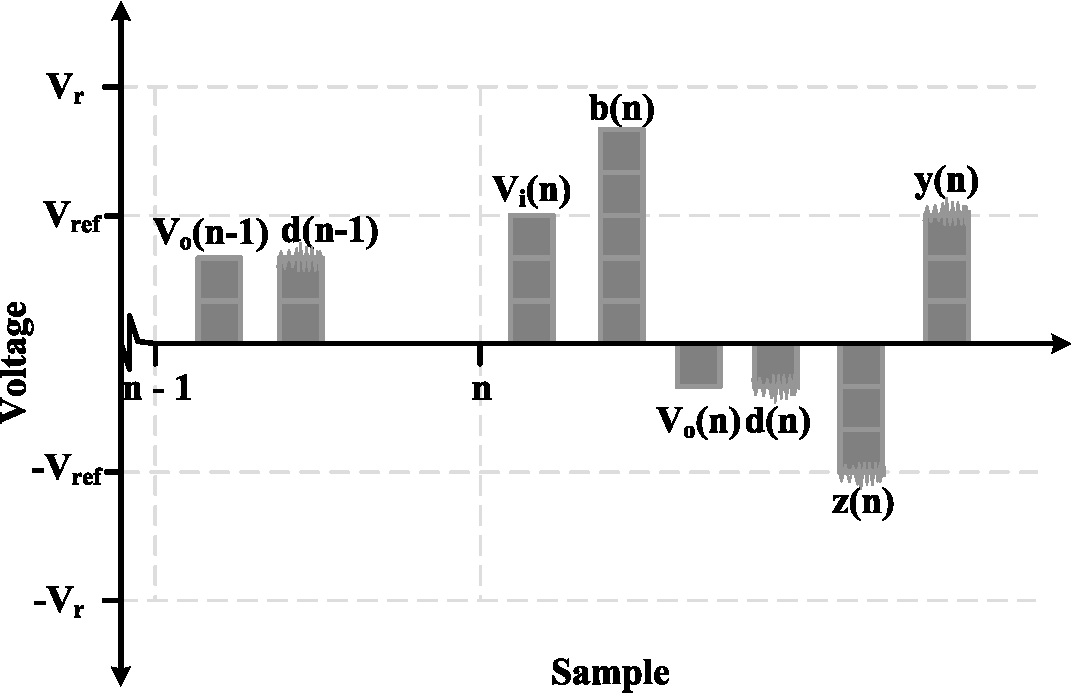
\includegraphics[width=\myfigwidth]{graphics/example}
%  \caption{Example of the modulator operation}
%  \label{p3fig:example}
% % \end{minipage}
%\end{figure}

%-------------------------------------------------------
\section{The Analog Modulo Integrator} \label{p3modint}
%-------------------------------------------------------
As shown, the modulo integrator is an integrator that resets when the output
increases or decreases beyond a reference voltage. It keeps the remainder that exceeds the reference voltage. A requirement set on the analog modulo integrator is that it should use maximum
swing available, for example 0.8V peak-to-peak with 1.2V supply. It should also be
a discrete time system. The discrete time equation for a
modulo integrator was shown in \req{modint}.

Using pseudo code the modulo integrator can be described as
\begin{enumerate}
\item Add the previous output to the current input
\item If the new output exceeds the reference voltages
\item Subtract/Add the range of the integrator, $V_r$ 
\item Set the current output to the remainder
\end{enumerate}

This is trivial to implement in the digital domain, but it may not be obvious how it
should be implemented in the
analog domain. Adding two voltages in the analog domain is conceptually
trivial. Whether a voltage exceeds a reference can be detected using a
comparator. Subtraction in the analog domain is also trivial, but
keeping the remainder presents a challenge. 

Assume that the reference voltages are
symmetric around the common mode, such that $|V_{ref}| =
|-V_{ref}|$ and $|V_{ref}|+ |-V_{ref}| = V_r$. The maximum voltage
would be less than $V_{ref} + V_{ref} = V_r$ or more than $-V_{ref} + -V_{ref} = -V_r$.  So the output after
summation, but before modulo operation, will be bounded by
\eqn{
\label{p3eq:brange}
-V_r < b(n) < V_r
}
In a circuit where the analog value is represented by voltages the swing would have to be $2V_r$ to
accuratly represent all analog values. Since our input signal has a range
of $V_r$ we would waste an extra range of $V_r$ just to represent
intermittent values in the integrator. It would be best if we could
set the voltage swing of the circuit to $V_r$, which is equal to the
maximum input swing. But in a circuit where the analog values are
represented with voltages this is difficult.

%-------------------------------------------------------
\subsection{A Solution Based on Switched Capacitors}
%-------------------------------------------------------
Switched-Capacitor (SC) circuits are prevalent in many analog
integrated circuits. In discrete time Sigma-Delta modulators it is common to
implement the integrator with a switched-capacitor circuit. It turns out that with small
modifications a switched-capacitor integrator can be converted to an analog modulo integrator. 

Realizing that in a switched capacitor integrator the analog value is
stored as charge and not as voltages is the key to understanding how a
modulo integrator can be implemented. A conventional
switched-capacitor integrator, shown in Figure \ref{p3fig:integrator}, adds the previous
output and current input. When the
integrator has settled, or failed to settle due to saturation of the opamp, it can be detected whether the output voltage
exceeds the reference voltage. If it does exceed, a charged capacitor is connected to
the charge transfer node of the integrator, node $V_g$ in Figure \ref{p3fig:integrator}. This subtracts/adds the charge
which represent $V_r$. Provided that the input signal
to the integrator never exceeds positive or negative reference, the
subtracted/added charge will bring the integrator back within bounds. Since the analog information is
stored in charge, the remainder is conserved. 

\begin{figure}[ht]
\centering 
 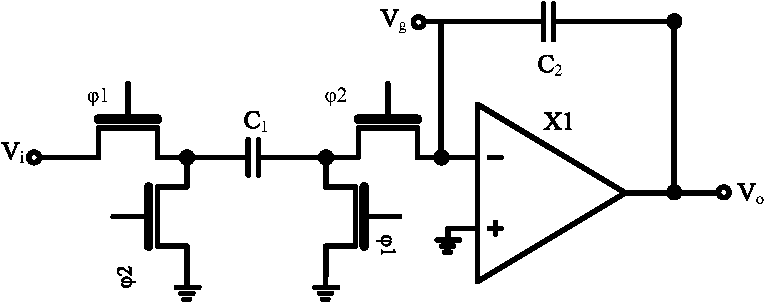
\includegraphics[width=\myfigwidth]{graphics/integrator}
  \caption{Conventional Switched-Capacitor Integrator}
  \label{p3fig:integrator}
\end{figure}

%-------------------------------------------------------
\subsection{Equations of the SC Modulo Integrator}
%-------------------------------------------------------

The circuit needed to implement a modulo integrator is shown in Figure
\ref{p3fig:moddetector}. It is connected to integrator in node $V_g$ and
$V_o$.
The complete circuit has
three clock phases; $\phi 1$, $\phi 2$ and $\phi 3$. The timing
diagram is shown in Figure \ref{p3fig:timing}, where $T$ denotes the period. 

%The analog modulo integrator can be compared to
%a first-order LC-SDM with one integrator, 1.5 bit quantizer
%and a 1.5 bit DAC. However, in the analog modulo integrator it is not the output from
%the quantizer (comparators X2 and X3 in Figure \ref{p3fig:moddetector} )
%that is used, but the analog output of the
%integrator. 

\begin{figure}[ht]
\centering 
 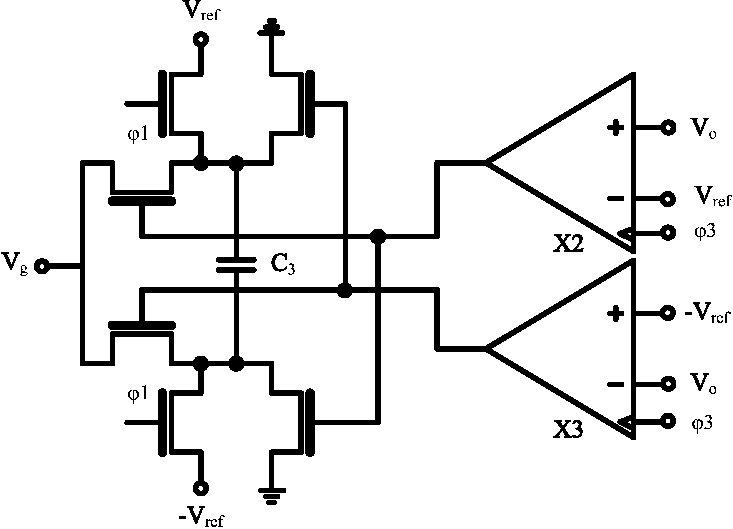
\includegraphics[width=\myfigwidth]{graphics/moddetector}
  \caption{Modulo circuit}
  \label{p3fig:moddetector}
\end{figure}

\begin{figure}[ht]
\centering 
 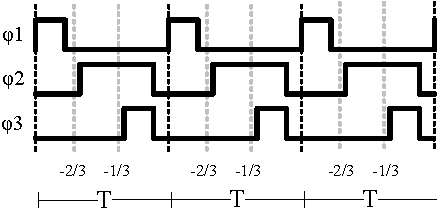
\includegraphics[width=\myfigwidth]{graphics/timing}
  \caption{Timing diagram for the modulo integrator}
  \label{p3fig:timing}
\end{figure}

Consider the integrator in Figure \ref{p3fig:integrator}, during clock phase $\phi 1$ the
input signal is sampled across capacitor C1. In clock phase $\phi
2$, before $\phi 3$, the charge from C1 is transfered to C2. The charge transfer
equation will be 
\eqn{
\label{p3eq:chargetf1}
C_2V_o(n-T/3) = C_2V_o(n-T) + C_1V_i(n-2T/3)
}
In this equation the output, $V_o(n-T/3)$, is equivalent to
$ b(n)$ from \req{modintb} and will have the same bounds, assuming $C_1 = C_2$. To make sure that the final
output, $V_o(n)$, stays within the reference voltages, $V_r$ has to be
added or subtracted as in \req{modint}.

To perform the addition/subtraction the circuit in Figure
\ref{p3fig:moddetector} is used. The different states of this circuit are
shown in Figure \ref{p3fig:moddetexpl}. During $\phi 1$, Figure
\ref{p3fig:moddetexpl} a), the capacitor $C_3$ is charged to $V_r =
V_{ref} - -V_{ref}$. During $\phi 3$ the latched comparators ( $X2$
and $X3$ in Figure \ref{p3fig:moddetector})
determine whether the output voltage exceeds the reference. Figure
\ref{p3fig:moddetexpl} b) shows the connections if the
output voltage, $V_o(n-T/3)$, is higher than $V_{ref}$. Here a charge
of $Q_3 = C_3V_r$ is transfered to the node $V_g$ in the
integrator. This will change the charge transfer equation into
\eqn{
\label{p3eq:chargetf2}
C_2V_o(n) = C_2V_o(n-T) + C_1V_i(n-2T/3) - C_3V_r
}
For $V_o(n-T/3)$ lower than $-V_{ref}$, Figure \ref{p3fig:moddetexpl}
c), the polarity of the charge is reversed and the charge transfer
function is
\eqn{
\label{p3eq:chargetf3}
C_2V_o(n) = C_2V_o(n-T) + C_1V_i(n-2T/3) + C_3V_r
}
And if $-V_{ref} < V_o(n-T/3) < V_{ref}$ the capacitor $C_3$ is not
connected to $V_g$ and the charge transfer function \req{chargetf1}
remains unchanged. Notice that the outputs from the comparators can
never be high at the same time, because $V_o(n-T/3)$ cannot be higher
than $V_{ref}$ and lower than $-V_{ref}$ at the same time.

Combining the three equations,
\req{chargetf1}, \req{chargetf2} and \req{chargetf3} with $C_1 = C_2 = C_3$ and ignoring the
frational timesteps ( $n-T/3$ and
$n-2T/3$) the result is \req{modint}.

\begin{figure}[ht]
\centering 
 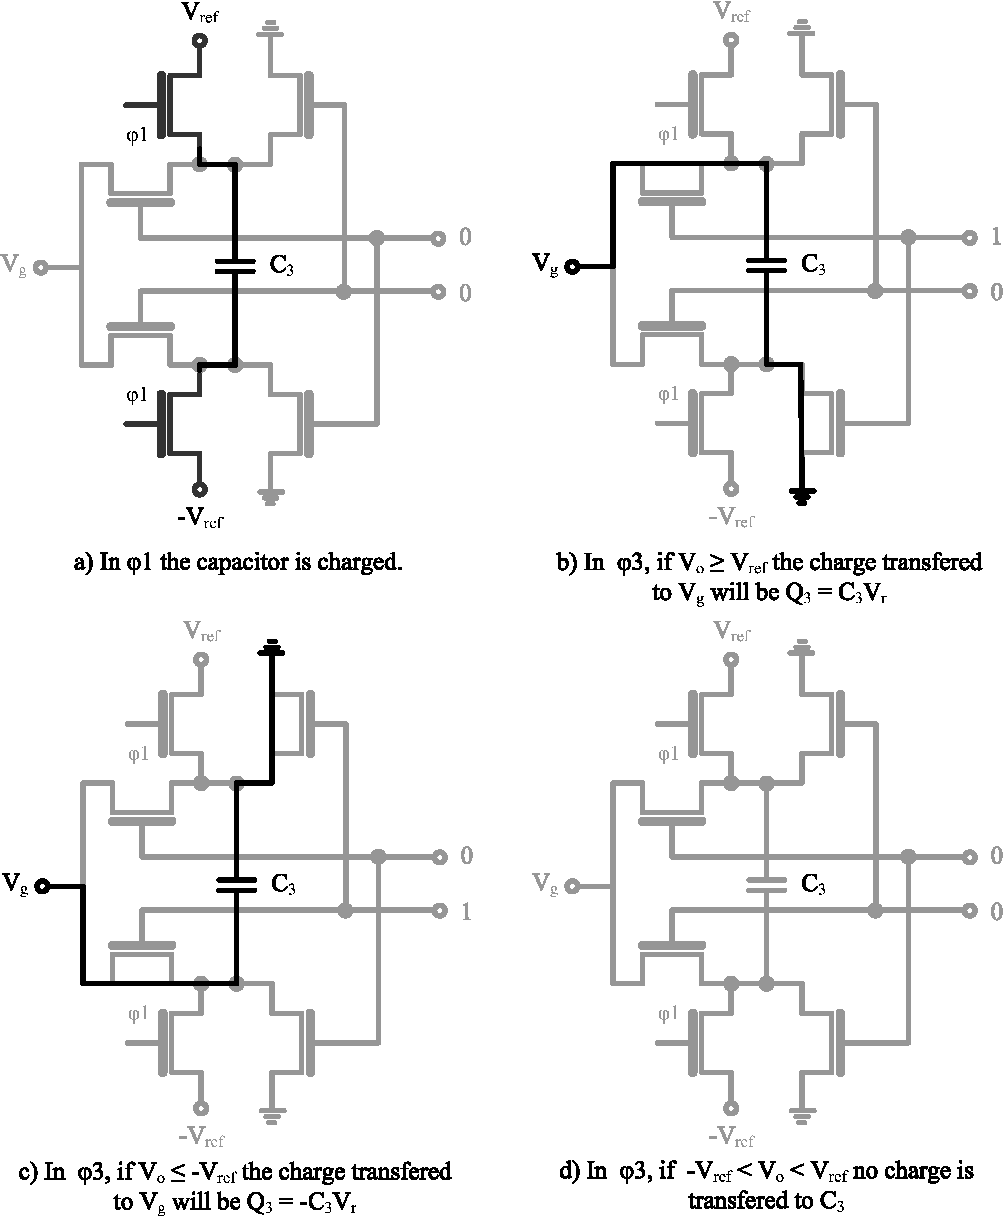
\includegraphics[width=3in]{graphics/moddetexpl}
  \caption{The different permutations of the modulo circuit}
  \label{p3fig:moddetexpl}
\end{figure}


%-------------------------------------------------------
\subsection{Simulation of the SC modulo integrator}
%-------------------------------------------------------
Simulation of the SC modulo integrator have been performed in
AimSPICE \cite{aimspice} using ideal models for comparators, switches
and operational amplifier. 

In Figure \ref{p3fig:modintdc} a DC input
signal $V_i = 0.3V$ was used, the reference voltages were set to 1V. At around $5 \mu$ the integrator
resets, here the output value would be $1.2V$ if it was not reset, and
we can clearly see that the remainder is conserved 
\eqn{-1 V + 0.2 V = -0.8V}

\begin{figure}[ht]
\centering 
 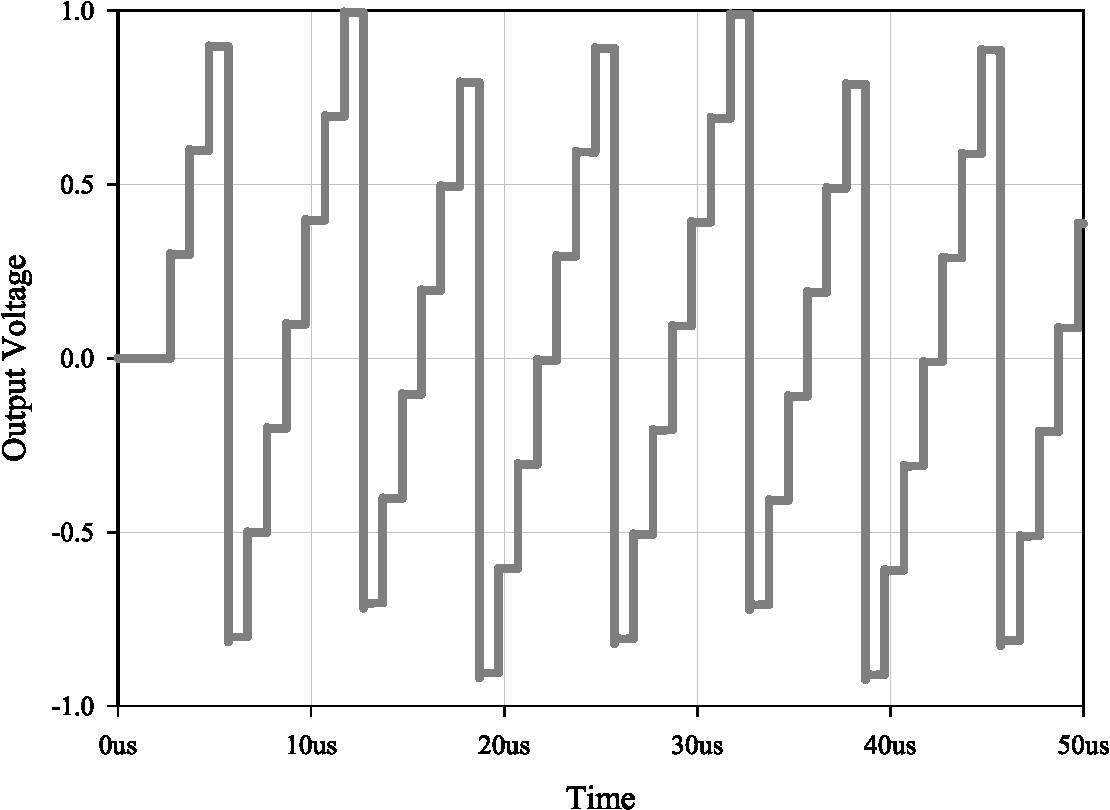
\includegraphics[width=\myfigwidth]{graphics/modintdc}
  \caption{Input vs output for the modulo integrator with constant input $V_i = 0.3V $}
  \label{p3fig:modintdc}
\end{figure}

In Figure \ref{p3fig:modintsine} the input and output for a sinusoidal
input to  the analog   modulo integrator is shown. The reference
voltage, $V_{ref}$, was set to 1V.
The sinusoidal input had an amplitude of $0.99 V$. The output has
been sampled at the end of $\phi 3$ and it can be seen how it never
exceeds the references at $V_{ref}$ and $-V_{ref}$.



%Figure \ref{p3fig:modintsine} shows the output, $V_o$, of the integrator


\begin{figure}[ht]
%  \begin{minipage}[b]{\myfigwidth}
\centering 
 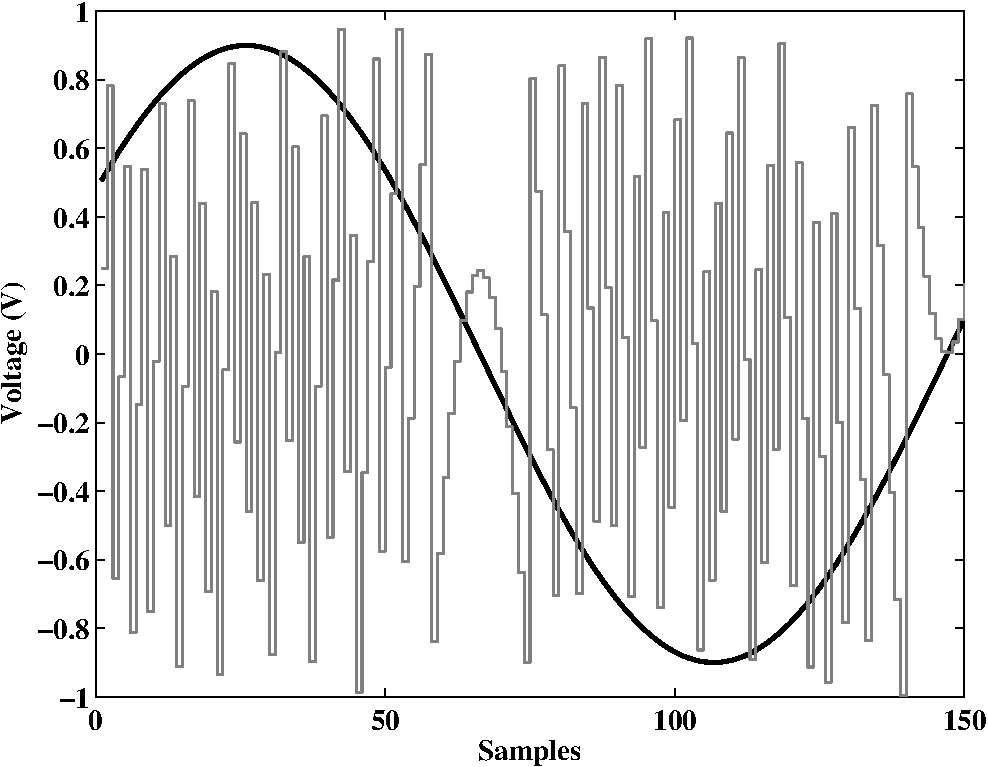
\includegraphics[width=\myfigwidth]{graphics/modintsine}
  \caption{Input vs output for the modulo integrator. Input is a sine
  with an amplitude of 0.99 V}
  \label{p3fig:modintsine}
 % \end{minipage}
\end{figure}

%-------------------------------------------------------
\section{Simulation of OLSDM Modulator}\label{p3simulation}
%------------------------------------------------------- 
The OLSDM was modeled in SystemDotNet \cite{systemdotnet05}, which is a
mixed-signal discrete-time event driven simulator. A third order
OLSDM with 8 bit quantizer was modeled. The spectral density plot can
be seen in Figure \ref{p3fig:simolsd}. From the plot we can clearly see
that we have third order high-pass filtering of the quantization
noise since the slope of the noise floor is 60dB per
decade. The dark-gray plot is an oversampled quantizer without noise
shaping, shown for comparison. With an
oversampling ratio of eight we get an ENOB (Effective Number
  Of Bits) of 15 bits. With just oversampling, no noise shaping, we
get an ENOB of 9.5 bits. 

\begin{figure}[ht]
%  \begin{minipage}[b]{\myfigwidth}
\centering 
 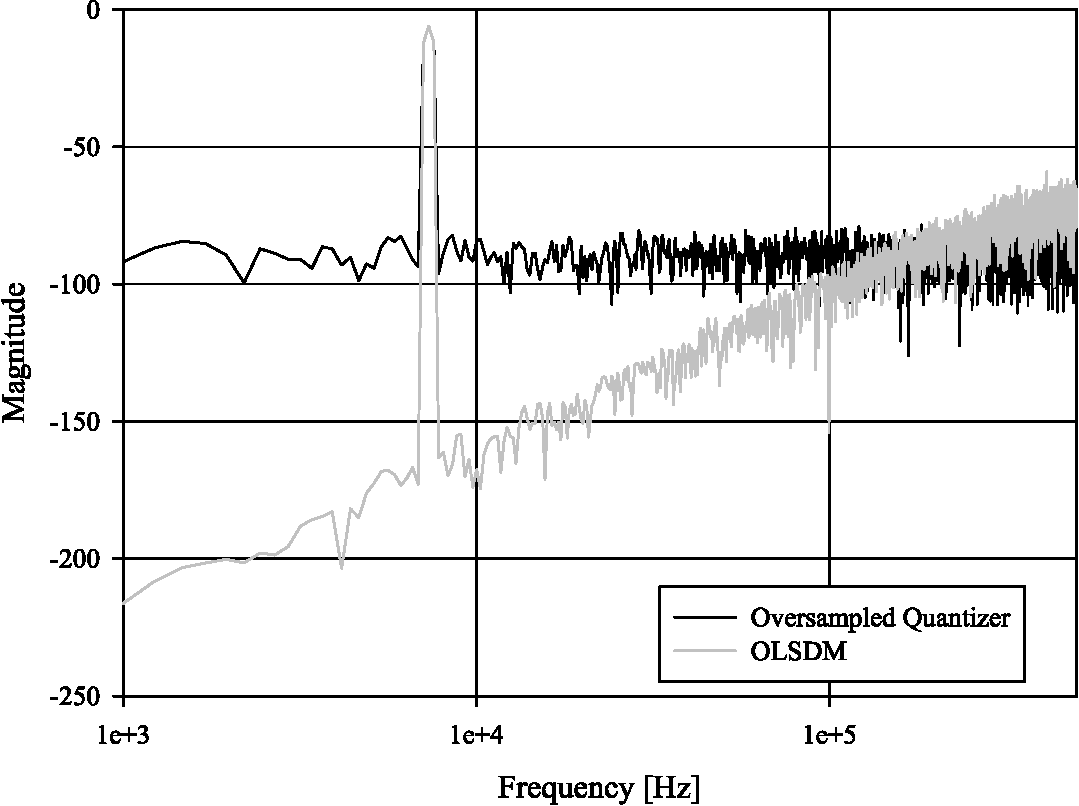
\includegraphics[width=\myfigwidth]{graphics/simolsd}
  \caption{Simulation of third order, 8 bit OLSDM. Input signal
  amplitude is $0.5$ and sampling frequency is 1MHz. Also shown is the
  output from a oversampled quantizer without noise shaping }
  \label{p3fig:simolsd}
 % \end{minipage}
\end{figure}

The analog modulo integrator can be compared to a first
order, 1.5 bit LC-SDM. In Figure \ref{p3fig:simmodint} we have
plotted the output from the OLSDM  and the combined outputs from the
comparators in the analog modulo integrator (outputs of X2 and X3 in
Figure \ref{p3fig:moddetector}). We
can clearly see that the combined output of the comparators is a first order
noise shaped version of the input signal. One could summize
that the analog modulo integrator is just a 1.5 bit LC-SDM, but that
would be inaccurate. If we assume the input signal is bounded by
\req{rangeinput}, the analog modulo integrator output will never
exceed $-V_{ref}$ or  $V_{ref}$, altough the output during $\phi2$
might saturate. For the LC-SDM the input signal swing is
normally reduced such that the output of the integrator does not
saturate.

\begin{figure}[ht]
\centering 
 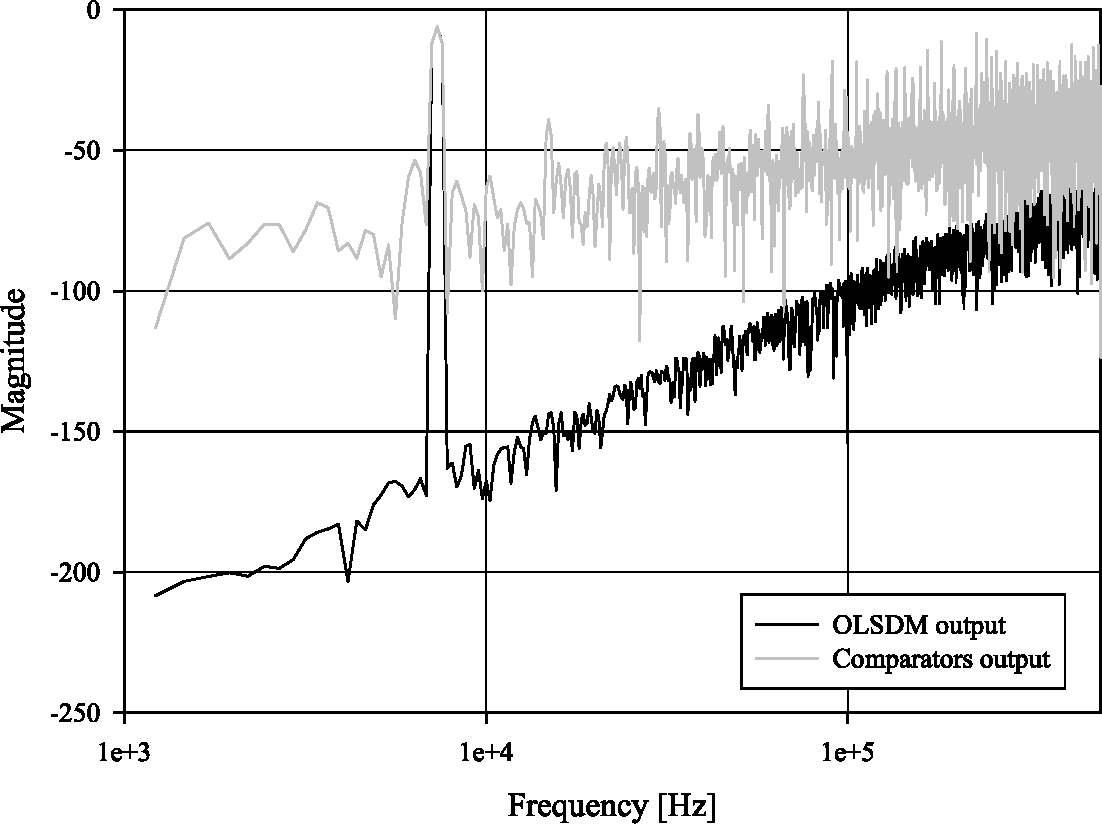
\includegraphics[width=\myfigwidth]{graphics/simmodint}
  \caption{The combined output of the comparators and the output of the OLSDM}
  \label{p3fig:simmodint}
\end{figure}

%-------------------------------------------------------
\section{Future Work}
%-------------------------------------------------------
The OLSDM architecture with analog modulo
integrator is, to our knowledge, a new architecture. Thus there are many questions to be
answered and some questions that have not yet been asked. Research is
currently being performed on the effects of mismatch, finite opamp
gain, non-linearity of quantizer, finite number of bits in quantizer,
and effects of parasitics. We hope to have an answer to some of these
questions in the near future.  
 
%-------------------------------------------------------
\section{Conclusion}
%-------------------------------------------------------
A switched-capacitor analog modulo integrator was presented. This analog modulo
integrator made it possible to design  
an Open-Loop Sigma-Delta Modulator (OLSDM). The theory of OLSDM and
analog modulo integration was explained and verified through simulation.

%------------------------------------------------------------------------
\section*{Acknowledgments}
%------------------------------------------------------------------------
{\small Financial support from the Norwegian Research Council through the
project Smart Microsystems for Diagnostic Imaging in Medicine (project
number 159559/130) and the project ASICs for Microsystems (project
number 133952/420) is gratefully acknowledged. }

%-------------------------------------------------------
%Figures
%-------------------------------------------------------


